\section{Evolutionsalgoritmer}
% Kort forklaring af at det er dette emne vi har valgt at arbejde videre med.
Analysen af tilgange til at modellere sværme, har ledt til en beslutning om at arbejde videre med evolutionsalgoritmer. Derfor er det nødvendigt at undersøge denne tilgang nærmere, for at finde den rette tilgang til en løsning. I dette afsnit forklares nogle underkategorier og tilhørende termer, mere dybdegående. På baggrund af denne yderligere analyse, udvælges en fremgangsmåde.
\todo[inline]{}

\subsection{Genetiske algoritmer} 
Genetiske algoritmer er en af de mest brugte typer af evolutionsalgoritmer  \citep{genetic-algorithms}\citep{evolutionary-computing}. Disse algoritmer bruger de genetiske operatorer (Som beskrevet i afsnit \ref{subsec:Evolutionsalgoritmer}), til at finde en løsning på et problem (Flowchart for processen kan ses på figur \ref{Genetisk algoritme}). Løsningen vil ikke nødvendigvis være helt optimal, men algoritmerne anvendes oftest inden for områder, hvor det ville være upraktisk at afsøge hele udfaldsområdet, fordi det ville tage lang tid, og derfor er en approksimation af en optimal løsning godt nok. 
\par
% Forklarer hurtigt hvad kromosomer er
Algoritmen starter med at danne en befolkning af et bestemt antal agenter (mulige løsninger), som består af kromosomer. Disse kromosomer beskriver egenskaber ved agenten, såsom hvor meget den kan se, hvor hurtigt den kan accelerere og stoppe, hvor stor den er, mv. De kan være indkodet på forskellige måder, såsom en binær streng, et array af værdier, en streng af bogstaver eller en vektor. Det er på disse kromosomer, at de genetiske operatorer anvendes. 
%%%%%
\begin{figure}[H]
    \centering
    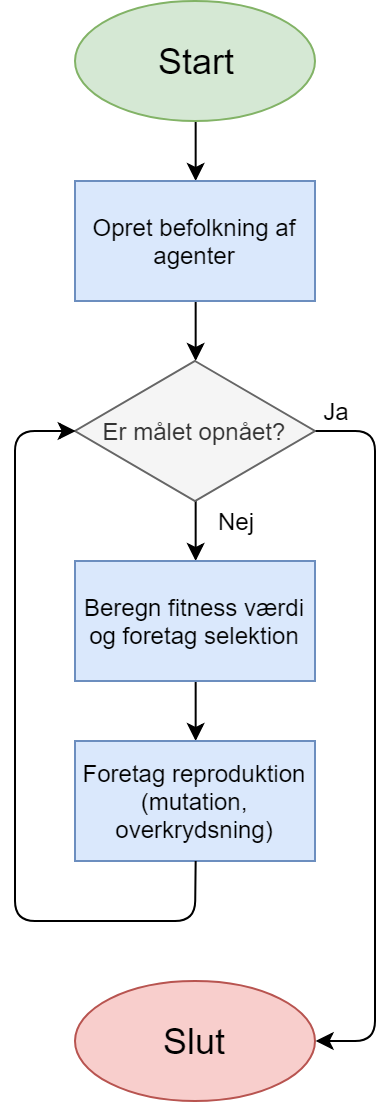
\includegraphics[width=0.27\textwidth]{figures/Genetisk_algoritme.png}
    \caption{Her ses en gennemgang af en typisk genetisk algoritme, som den ser ud uden yderligere tilføjelser \citep{evolutionary-computing}.}
    \label{Genetisk algoritme}
\end{figure}
%%%%%
% Forklarer selektion, kunne godt være dybere
Fitness-funktionen itererer over befolkningen af agenter og giver hver agent en fitness-værdi, alt efter hvor godt de klarede sig. Herefter kommer selektionen i spil, og udvælgelsen kan foregå på flere forskellige måder. En af måderne det kan gøres på, er at tildele hver agent en sandsynlighed for at blive udvalgt til at reproducere, baseret på deres fitness-værdi. Altså vil de agenter der har klaret sig bedst, have en større chance for at få lov til at reproducere. Denne fremgangsmåde kan ses som et roulette-hjul, hvor antallet af gange hver agent har en plads på roulette-hjulet, er relateret til deres fitness-værdi.
\par
% Forklarer overkrydsning
De agenter der udvælges til reproduktion (forældrene), bliver sat sammen, og det er her, overkrydsningen sker. Dette kan også gøres på flere forskellige måder, alt efter hvordan kromosomerne er indkodet, dog kan principperne overføres til alle mulige former for indkodning. Hvis kromosomerne eksempelvis er indkodet som binære strenge, kunne et punkt på kromosomet vælges, og den første del af den ene forældres kromosom splejses sammen med den sidste del af den anden forældres kromosom. En anden mulighed kunne være at vælge to punkter på kromosomet, og tage det der er imellem punkterne fra den ene forælder, og det der er uden for punkterne fra den anden forælder, og sætte det sammen. En sidste mulighed kunne være at hvert gen i kromosomet, eksempelvis hver bit, gennemgås, og algoritmen vælger hvilken forælder hvert gen skal komme fra, tilfældigt. Figur \ref{Overkrydsning} illustrerer disse tre eksempler på overkrydsning.
%%%%%
\begin{figure}[H]
    \centering
    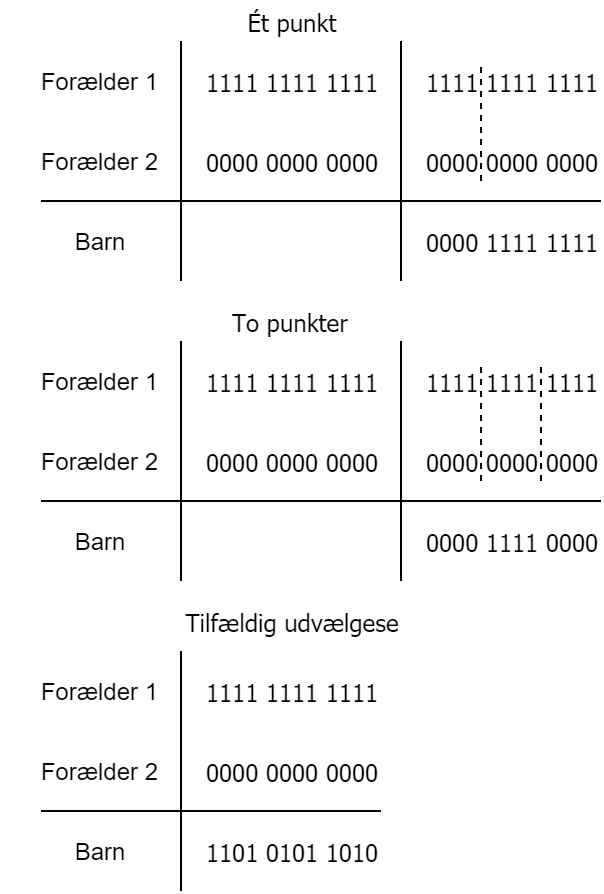
\includegraphics[width=0.5\textwidth]{figures/Overkrydsning.png}
    \caption{Eksempler på overkrydsning: ét-punkts, to-punkts og tilfældig overkrydsning.}
    \label{Overkrydsning}
\end{figure}
%%%%%
% Forklarer mutation
Ud af overkrydsningen kommer et barn, der har arvet egenskaber igennem et kromosom, der er sammensat af to eller flere forældres kromosomer. Efterfølgende kan mutation finde sted. Her kan programmøren definere en sandsynlighed for at en eller flere af værdierne i barnets kromosom defineres tilfældigt. Dette sørger for, at befolkningen forbliver varieret, så det er muligt for modellen at udvikle den bedste løsning.
\par
Barnet bliver en del af befolkningen i næste generation. Denne proces gentages, indtil der er lavet en ny generation med samme befolkningsantal som den gamle. Denne generation gennemgår så de samme mekanismer som deres forældre, og det fortsætter, indtil fitness værdien bliver høj nok, og målet er nået.
\par
% Forklarer hvorfor variation er vigtigt
Når der arbejdes med genetiske algoritmer er det vigtigt at have variation. Hvis variationen i befolkningen bliver for lav, kan modellen komme til at sidde fast i den forstand, at den ikke kan sammensætte forældre der er forskellige nok til at skabe et barn, der ikke er identisk med dets forældre. Dette kan betyde, at modellen når et plateau langt før den optimale løsning er fundet, hvis variationen havde været højere (Se figur \ref{GA plateau}). Som sagt kan mutation hjælpe med at holde variationen høj, men mutationsraten må heller ikke være for høj. En forhøjet mutationsrate kan sætte hastigheden for læringen ned, og i værste tilfælde forårsage, at hele modellen bare handler tilfældigt, og ikke gør sig nogen erfaringer, da alle kromosomer vil være helt tilfældige ved overkrydsning, og nedarvningen stopper. 
\par
%%%%%
\begin{figure}[H]
    \centering
    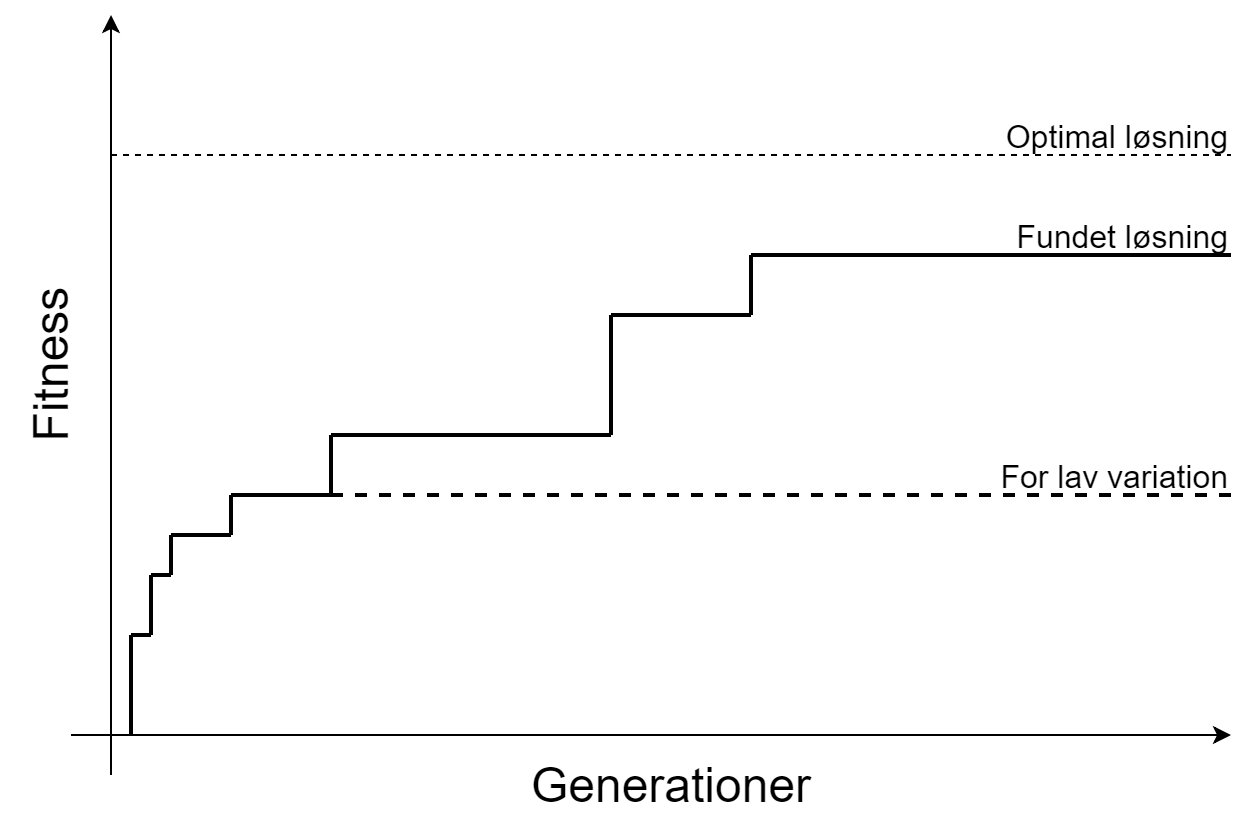
\includegraphics[width=0.9\textwidth]{figures/GA_plateau.png}
    \caption{Her ses en illustration af hvordan en for lav variation i befolkningen, kan påvirke det endelige resultat af en genetisk algoritme.}
    \label{GA plateau}
\end{figure}
%%%%%
% Mere om variation
En anden måde at afhjælpe en for lav variation i befolkningen, kunne være at gøre befolkningen større fra starten. Dette ville betyde, at befolkningen er mere varieret og mutationerne ville ske oftere, selv hvis mutationsraten er lav. Der ville derfor være større sandsynlighed for at generere en god løsning hurtigere. Befolkningen må dog ikke blive for stor, da det kan nedsætte hastigheden af simulationen. Det vil sige, at med en stor befolkning kan det være, at modellen kunne finde en god løsning ved at skabe halvt så mange generationer som ved en lavere befolkning, men hvis hver generation tager dobbelt så lang tid at simulere end en lavere befolkning, har man ikke vundet noget tidsmæssigt.
\par
% Afslutning
Denne type evolutionsalgoritme virker lovende, i og med at den kan bruges til at opbygge en model, der styrer individerne i sværmen. Der er dog det problem at algoritmen kræver en foruddefineret model den kan optimere, og denne model skal være baseret på reglerne for sværmen, som for så vidt er ukendte.


\subsection{Genetisk programmering}
% Forklarer forskelle mellem GA og GP. Resten af afsnittet tager udgangspunkt i at læseren ved hvad GA er.
Genetisk programmering drager ligesom den genetiske algoritme, inspiration fra evolutionen, ved at bruge mutation, overkrydsning, nedarvning og selektion, til at løse problemer. Ved genetisk programmering tænkes kromosomerne i stedet som et træ af instruktioner, frem for strenge af informationer \cite{genetic-algorithms}. De genetiske operatorer anvendes ikke på egenskaberne for hver agent, men på dette handlingstræ. Det vil altså sige at denne type algoritme ikke forsøger at optimere et program til at løse et problem, men i stedet forsøger at sammensætte selve programmet. 
\par
% Forklarer lidt mere om hvad genetisk programmering er
Programmøren skal altså kun definere hvilke mulige handlinger agenten kan foretage, og så skal algoritmen selv finde frem til hvilken rækkefølge disse handlinger skal foretages i. Dette sker som sagt ved hjælp af de genetiske operatorer, og foregår på samme måde som den genetiske algoritme, dog ved at bytte rundt på knuder i en træstruktur, frem for værdier i en tekststreng eller array (Se figur \ref{Tree_overkrydsning}). 
%%%%%
\begin{figure}[H]
    \centering
    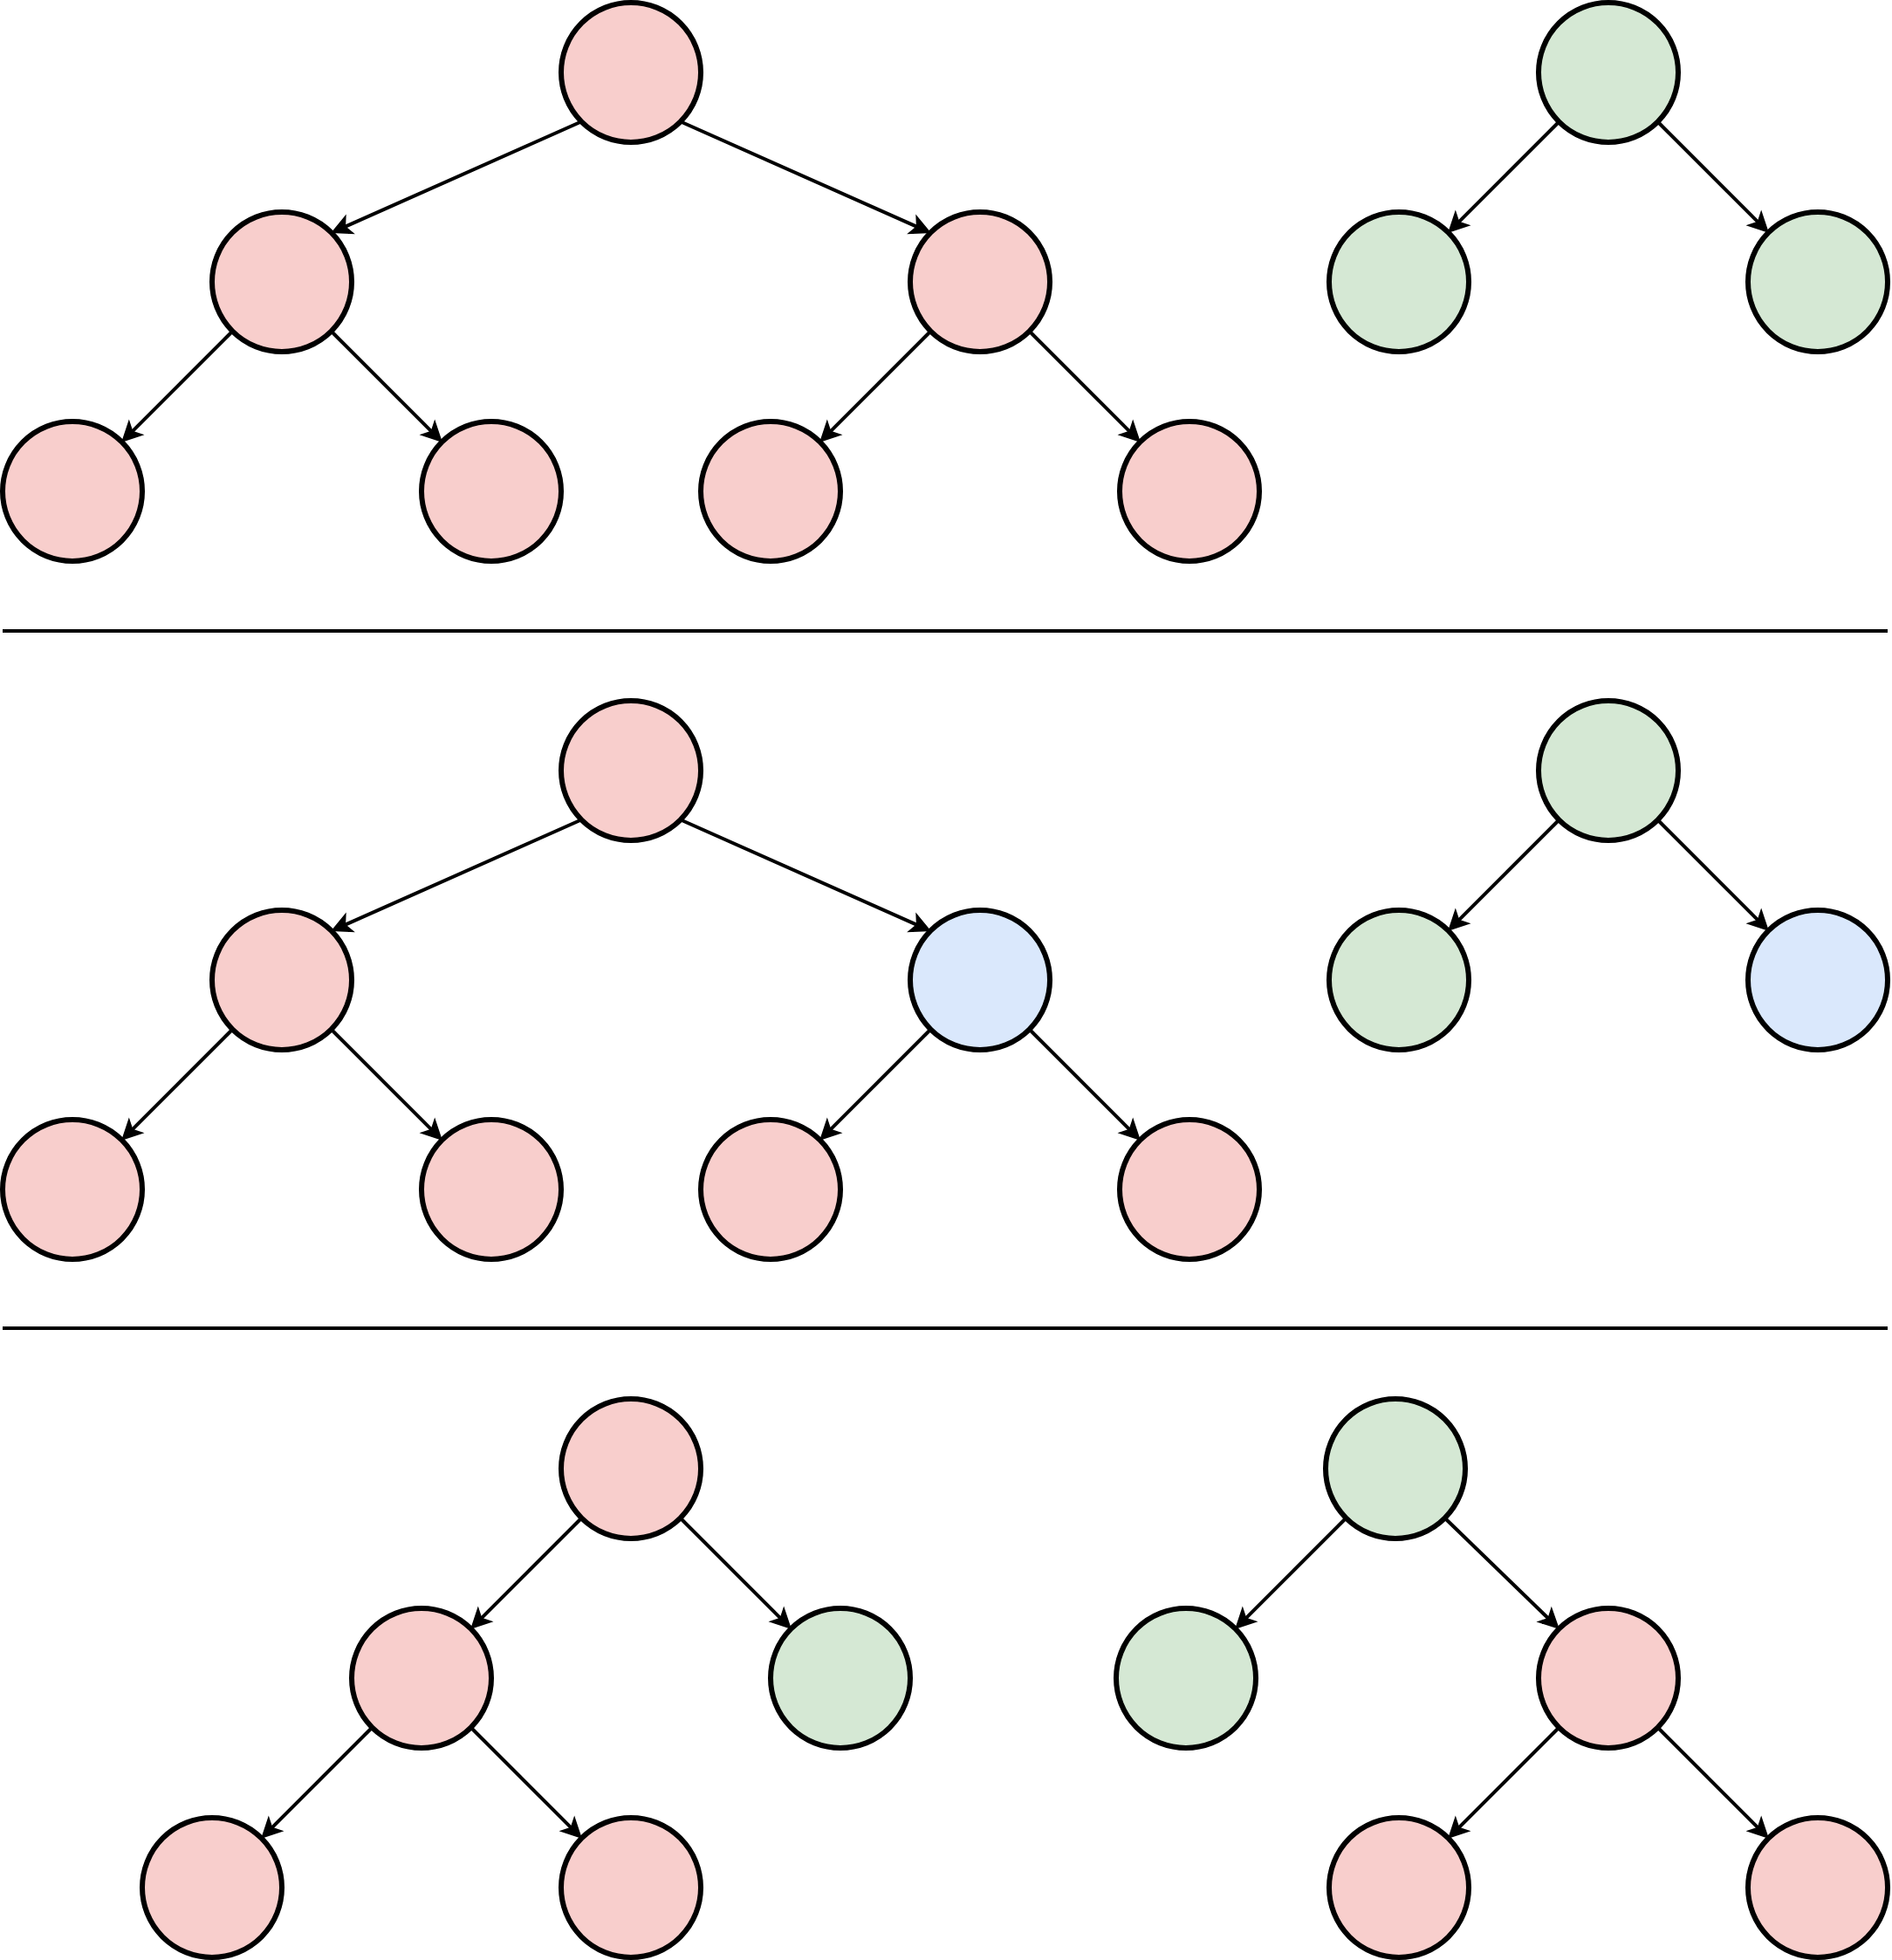
\includegraphics[width=0.5\textwidth]{figures/Overkrydsning2.png}
    \caption{To handlingstræer der gennemgår overkrydsning. Den blå farve markerer de to knuder der skal byttes ud, og alle deres underknuder følger med.}
    \label{Tree_overkrydsning}
\end{figure}
%%%%%
\par
% Forklarer hvorfor mutation ikke er så smart. Mangler måske CITATION
Mutation bruges ikke så ofte inden for genetisk programmering, da der kan opstå problemer, hvis en knude (node) i enden af handlingstræet muterer til en knude der skal have forgreninger for at kunne fungere, men ikke får nogen. Der kunne også forsvinde for meget information fra handlingstræet, hvis en knude i midten af træet muterer til en ende-knude, og træet derfor mister de knuder der var forbundet til den muterede knude (Se figur \ref{Tree_mutation}). Dette er ikke nødvendigvis dårligt for modellen, da det muligvis var den del der gjorde modellen dårlig, men det kunne også være en essentiel del af modellen som forsvinder. Problemet kunne også opstå ved overkrydsning, men der er det muligt at beholde al information, ved at lave to børn fra to forældre.
%%%%%
\begin{figure}[H]
    \centering
    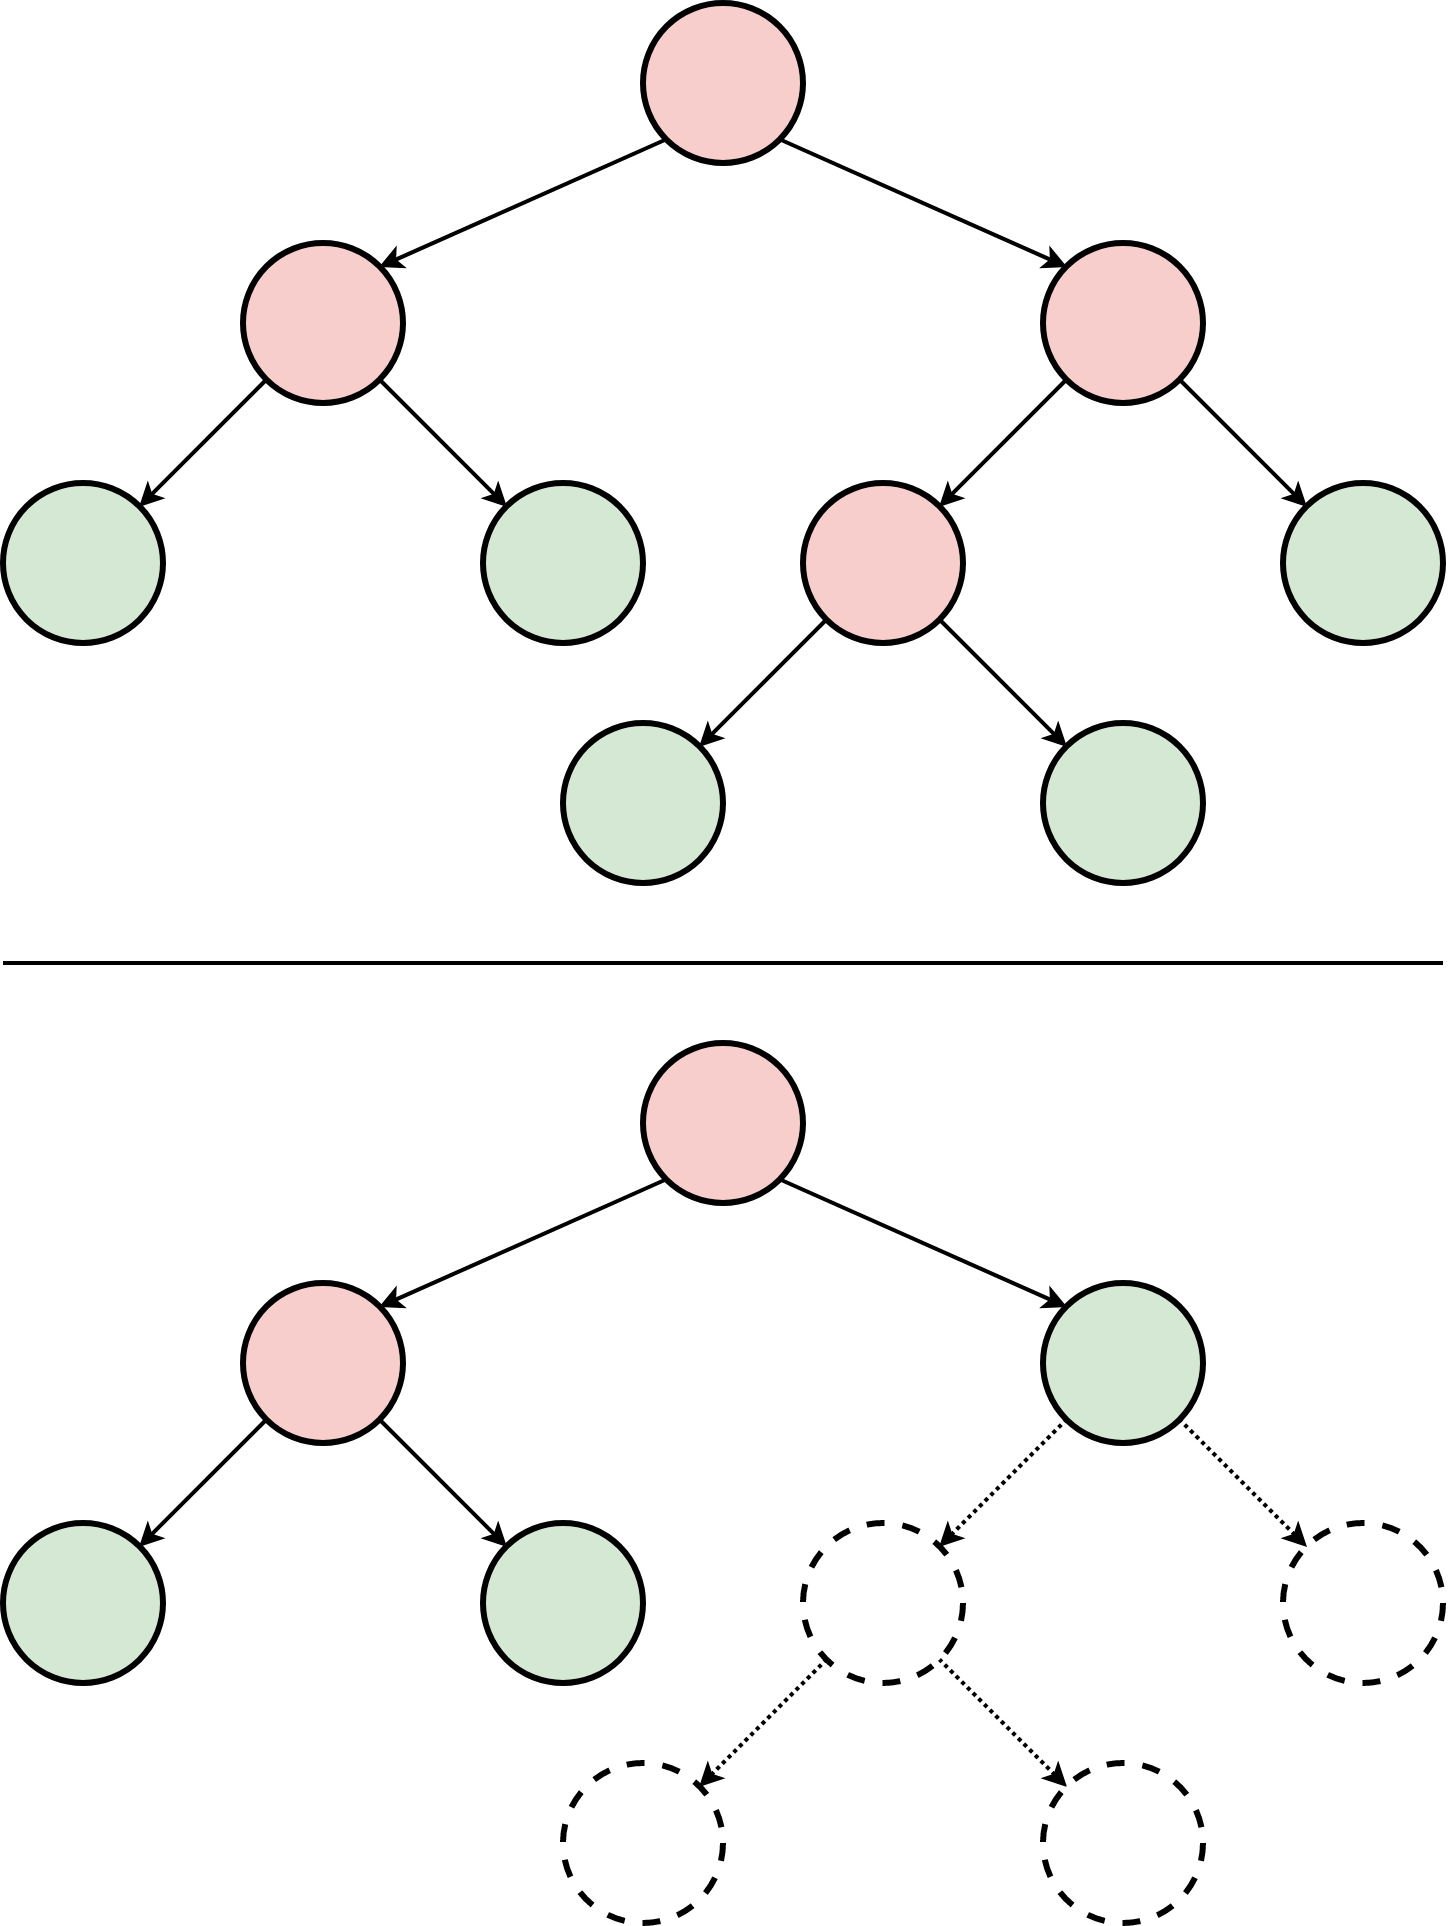
\includegraphics[width=0.4\textwidth]{figures/Mutation.png}
    \caption{Et handlingstræ mister muligvis for meget information ved mutation. De grønne knuder er ende-knuder som ingen forgreninger har.}
    \label{Tree_mutation}
\end{figure}
%%%%%
% Et eksempel på genetisk programmering. Forklarer hurtigt hvordan man skal læse figuren.
På figur \ref{Ant simulation} ses et handlingstræ for en myre der skal finde så meget mad som muligt, så hurtigt som muligt. Handlingstræet skal læses fra toppen, hvor myren checker om den kan se mad. Herefter udfører den alle handlingerne, indtil den har nået enden af træet, hvorefter den starter fra toppen igen. Dette bliver den ved med, indtil tiden udløber. Hvert "skridt"\ der tages i træet, tælles som et skridt frem i tid.
%%%%%
\begin{figure}[H]
    \centering
    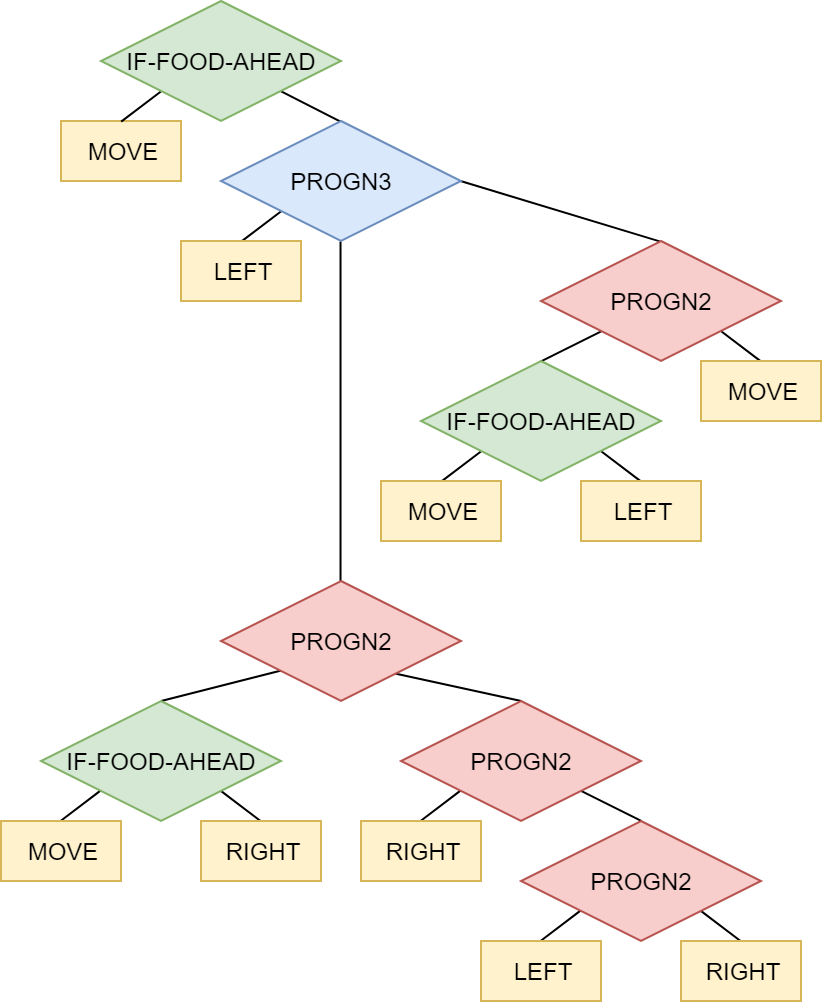
\includegraphics[width=0.6\textwidth]{figures/Ant_simulation.png}
    \caption{Handlingstræ for en simulation af en myre der leder efter mad i et gitter \citep{genetic-algorithms}. "IF-FOOD-AHEAD"\ er en if-sætning, hvor sand fører til venstre gren og falsk fører til højre gren. Dette knudepunkt aktiverer kun én af sine grene. "PROGN2"\ og "PROGN3"\ aktiverer alle deres grene fra venstre mod højre. "RIGHT"\ og "LEFT"\ drejer myren til henholdsvis højre og venstre, og "MOVE"\ skubber myren et skridt fremad.}
    \label{Ant simulation}
\end{figure}
%%%%%
% Forklarer mangler og problemer med GP
Dette handlingstræ er blevet udviklet ved brug af genetisk programmering, men det er ikke fejlfrit. De nederste to "PROGN2"\ kunne lige så godt erstattes med ét "RIGHT"\, da det eneste de gør, er at dreje myren til højre, så til venstre og så til højre igen. Dette er en ret uskyldig fejl, men den tager tid at afvikle, og det kunne løses ved at fitness-funktionen også belønnede korte handlingstræer. Dette tilføjer dog mere kompleksitet til fitness-funktionen, og den vil derfor også blive mere tidskrævende. En anden løsning kunne være manuelt at gennemgå det færdige handlingstræ, og finde de overflødige knuder.
\par
\todo[inline]{Mangler noget om simulering af mange individer}
\par
% Afslutning
Genetisk programmering virker som en god kandidat til at modellere sværme. Det er ikke nødvendigt at kende reglerne for hvordan agenter skal bevæge sig i en sværm, da algoritmen vil forsøge at finde frem til dem selv. Dog skal de handlinger hver agenter kan foretage, defineres på forhånd.


\subsection{Differential evolution}
% Skal lige have sat kilderne ind her.
Differentiel evolution (DE) er en metode der optimere et problem ved iterativt at forbedre en kandidatløsning. Disse metoder er også kendt som metaheuristikker, da de kun har få eller ingen formodninger om løsningen på problemet, og kan derfor søge i store mængder af kandidatløsninger, altså løsninger hvor agenten har en høj fitness-værdi. Dog er det ikke garanteret at en metaheuristik finder den optimale løsning. Et eksempel på en sådan optimering med DE er ”The 2d Ackley function”, som ses nedenunder på figur \ref{Ackley}.
%%%%
\begin{figure}[H]
    \centering
    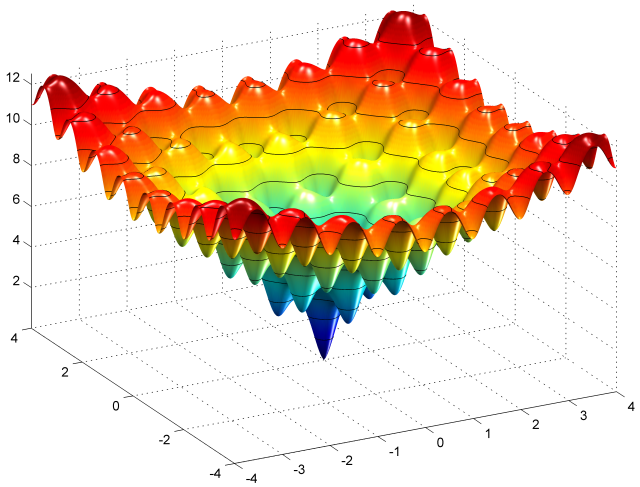
\includegraphics[width=0.6\textwidth]{figures/Ackley.png}
    \caption{En billede af hvordan \textit{Ackley funktionen} kan se ud. Agenterne vil her lede efter det globale minimum (0,0,0) ved at blive sat tilfældigt ind, og herefter bevæge sig rundt, og få en fitness-værdi efter hver bevægelse. Hvis værdien er acceptabel forbliver denne nye position, agtenens position, ellers vil agentens position blive sat tilbage til hvor den var før}
    \label{Ackley}
\end{figure}
%%%%
Funktionen prøver at finde det globale minimum igennem mange kandidatløsninger, funktionen vil dele problemet op i lokale problemer, og i dem prøve at finde et globalt minimum. Problemet er imidlertid, at den hurtigt kan komme til at sidde fast i et lokalt minimum og derfor aldrig finde det globale minimum. Ackley-funktionen bruges ofte som en test for at bedømme en optimeringsalgoritmes ydeevne. 
\par
DE bruges til multi-dimensionale funktioner, men bruger ikke gradienten af det problem der skal optimeres, hvilket betyder at det ikke er nødvendigt for DE at optimeringsproblemet er differentiabelt, i modsætning til nogle mere klassiske optimeringsmetoder som ”gradient descent” og ”quasi-newton methods”. DE optimerer et problem ved at opretholde en befolkning af kandidatløsninger, og samtidigt lave nye kandidatløsninger ved at kombinere de eksisterende løsninger på samme måde som ved genetiske algoritmer. 
\par
Selve DE algoritmen fungerer ved at den har en befolkning af kandidatløsninger (Agenter), som bevæger sig rundt i søgeområdet ved at bruge nogle relativt simple matematikske formler som kombinerer positionen af de eksisterende agenter (også kaldet mutation), og tager nogle tilfældige værdier fra de valgte agenter, og derved finder den nye position. Hvis den nye position af en agent forbedres, så accepteres den, og bliver en del af den allerede eksisterende befolkning. Denne proces gentages, og derigennem håbes det at den optimale løsning bliver fundet, men som tidligere nævnt, er det ikke en garanti at dette sker. Alt dette sker igennem fire faser, initiation, mutation, kombination og selektion.
%%%%
\begin{figure}[H]
    \centering
    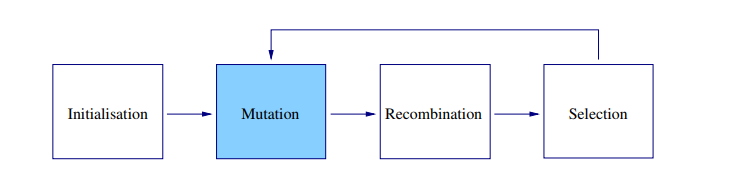
\includegraphics[width=0.8\textwidth]{figures/tur.PNG}
    \caption{Her ses det hvordan funktionen gennemgår de fire faser indtil de opsatte krav er opnået}
    \label{tur}
\end{figure}
%%%%
I en DE-funktion er der tre nødvendige parametre, differentielvægten , sandsynligheden for overkrydsning og befolkningens størrelse. Disse parametre kan have stor indflydelse på optimeringens ydeevne. Udvælgelsen af de bedste parametre er et emne der er blevet studeret rigtig meget, og de bedste metoder der er fundet er "Rules of thumb" som er fundet af (storn et al(find kilden)), matematisk konvergensanalyse fundet af (Zaharue(FIND KILDEN)) og "meta-optimering" fundet af (Pedersen og zhang et al(FIND KILDEN)).
(MANGLER KILDER)
% Skal lige have afsluttet her.